
\chapter[Chapter 1]
{Training Humanoid Gaits using Reinforcement Learning and Rapid Motor Adaptation}
%\footnote{This is a sample for chapter footnote.}}
%\vspace{-7ex}
% \author{Nithin Chalapathi}
% \author{Yiheng Du}
% \author{Sanjeev Raja}
% \author{Aditi S. Krishnapriyan}

\address{\orgdiv{University of Colorado, Boulder}, 
\orgname{EECS and Chemical Engineering}, 
\postcode{94720},
     \city{Berkeley}, \country{United States of America}}%

%\address[2]{\orgdiv{Lawrence Berkeley National Laboratory}, 
%\orgname{Applied Mathematics and Computational Research Division}, 
%\postcode{94720}, 
%     \city{Berkeley}, \country{United States of America}}%

%\address[3]{\orgdiv{II Author Organization Division Name}, 
%\orgname{Organization Name}, 
%\postcode{Postal Code}, \countrypart{Part of the Country}, 
%     \city{City Name}, \street{Street Name}, \country{Country}}%

\author{Niraj Pudasaini and Nikolaus Correll. Corresponding author: \email{niraj.pudasaini@colorado.edu}}

\maketitle
%This tag is required to print author and address in the output
\vspace{-8ex}

\begin{abstract}{Abstract}

The rapid success of machine learning 
%in various fields has sparked significant interest in applying and developing techniques to scientific spatial and temporal modeling. This has led to the development of the field known as physics-informed machine learning (PIML). Physics-informed machine learning integrates traditional scientific modeling with modern data-driven techniques to enhance the understanding and prediction of complex systems across scientific and engineering domains. While traditional machine learning excels at pattern recognition and prediction from large datasets, it often operates independently of the physical principles governing the systems. Conversely, physical models offer high interpretability and reliability but struggle with real-world data complexity. PIML aims to address these limitations by combining the strengths of both approaches, promising improved accuracy, generalization, and scalability.  
% This chapter discusses different facets of physics-informed machine learning including data generation, current architectures, training objectives, open problems, and the role of scaling in handling larger datasets and complex models.
\end{abstract}

%\begin{abstract}{}
%Abstract text. Abstract text. Abstract text. Abstract text. 
%\end{abstract}

\keywords{physics-informed machine learning, neural networks, physics-constrained objectives}

\begin{figure}[H]
    \centering
    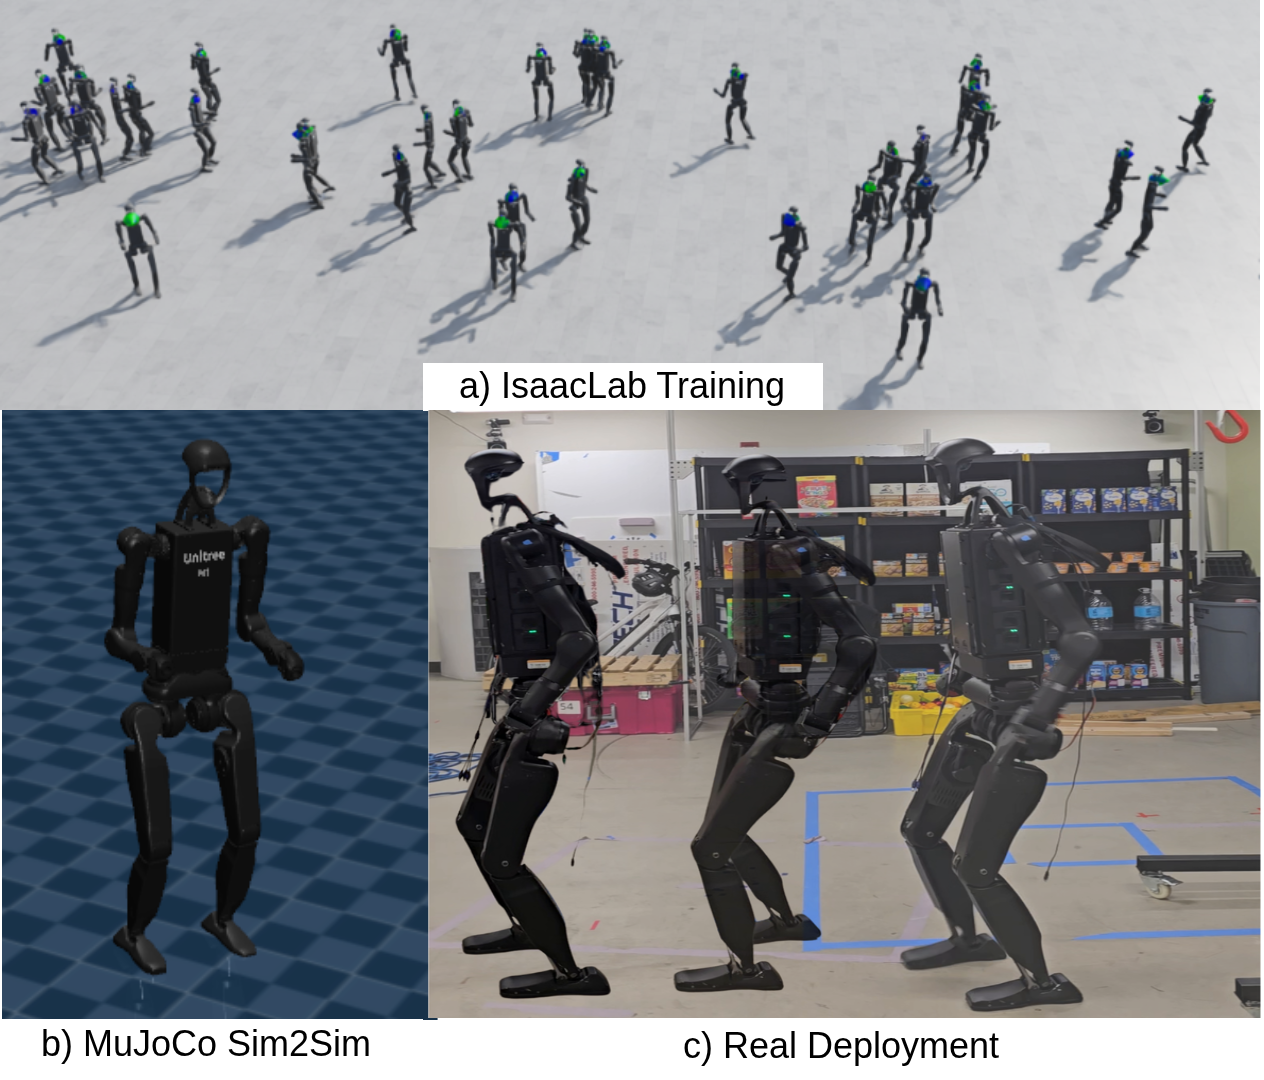
\includegraphics[width=1.0\linewidth]{figures/book_chapter_diagram.png}
    \caption{(a) IsaacLab training: large-scale parallel simulation. (b) MuJoCo sim2sim: the learned policy and robot model are replayed in another simulator. (c) Real deployment: transferring the learned gait real hardware.}
    \label{fig:training_inference}
\end{figure}


\section{Introduction}

Humans move through diverse environments easily, using just two legs to walk, turn, climb, and adapt to a wide variety of terrains. Inspired by this natural efficiency, bipedal robots aim to replicate human-like mobility. In comparison to wheeled or tracked robots, which are made for planar surfaces, bipedal robots are capable of navigating uneven, cluttered terrains, and even stepping over obstacles. Yet mobility alone does not make a humanoid useful. It must interact with its environment such as lifting objects, pulling doors, carrying loads, which involve sustained physical contact and forceful bimanual manipulation. This chapter addresses both challenges: teaching a humanoid to walk and teaching it to remain stable for bi-manual manipulation.

% Moreover, humanoid robots are designed to operate in human-centered environments, where interaction with human tools and existing infrastructure is required. Bipedal locomotion allows humanoid robots to perform a range of tasks and generalize across real-world environments designed for humans.

Traditionally, researchers have addressed the problem using model-based methods, which have been in existence since the 1980s \citep{Gupta18062017,reher2020dynamicwalkingagileefficient}. Initial research relied on highly simplified models, such as the Linear Inverted Pendulum Model (LIPM) \citep{6697099}, which reduced the complexity of bipedal dynamics to make control and theoretical analysis more tractable. As research progressed, advanced methods such as model predictive control (MPC) \citep{machines10110975, li2022dynamicwalkingbipedalrobots, Herzog_2016} and Trajectory Optimization (TO) \citep{li2018usingdeepreinforcementlearning, 9206554} are used, where robot dynamics is explicitly modeled, and trajectories or control policies are optimized subject to constraints such as balance, torque limits, and stability of ground contact. For example, whole-body controllers have been developed based on quadratic programming formulations to handle contact-rich dynamics and prioritize multiple tasks \cite{1241826,article}. Similarly, TO approaches have been applied to generate dynamically stable walking gaits \cite{4115592, 7487270}. Although model-based methods converge quickly and provide strong predictability, they tend to perform poorly in highly dynamic and uncertain settings where flexibility and adaptation are required.

Reinforcement learning (RL), and in particular deep reinforcement learning (DRL), has emerged as an alternative to learning control through policies with interaction in simulated environment rather than explicit analytical design \citep{schulman2017trustregionpolicyoptimization, schulman2017proximalpolicyoptimizationalgorithms, lillicrap2019continuouscontroldeepreinforcement, heess2017emergencelocomotionbehavioursrich}. Although often viewed as fundamentally different from model-based optimization, RL in practice also relies heavily on models, typically in the form of physics-based simulators. From this perspective, RL uses simulators to generate large-scale data, enabling learning-based optimization to discover control strategies that are difficult to design manually \citep{pmlr-v28-levine13, williams2015modelpredictivepathintegral}.

DRL has shown remarkable success in learning stable and agile locomotion behaviors, with early successes observed in quadruped robots \citep{doi:10.1126/scirobotics.aau5872, doi:10.1126/scirobotics.abc5986, tan2018simtoreallearningagilelocomotion}. While the underlying DRL algorithms, such as policy gradient and actor–critic methods remain largely unchanged when applied to bipedal humanoids, the transition to humanoid locomotion introduces substantially greater challenges due to increased morphological complexity, under-actuation, intermittent foot contacts, and stricter bipedal balance. As a result, learning stable humanoid locomotion typically requires more carefully shaped reward functions, richer state representations, and longer training horizons to capture whole-body coordination and dynamic balance. Recent work shows that DRL can produce robust and dynamically stable bipedal locomotion policies in simulation and that such policies can be successfully transferred to real humanoid robots \citep{gu2024humanoidgymreinforcementlearninghumanoid, doi:10.1126/scirobotics.adi9579, Singh_2024}.

Despite the success of DRL in simulation, the transfer of learned policies to real robot is challenging due to the simulation to reality gap, induced by discrepancies in real-world dynamics, sensing, and actuation \citep{10.1007/3-540-59496-5_337}. Broadly, prior work addresses this challenge through two complementary strategies: \emph{reducing} the reality gap or \emph{overcoming} it \citep{aljalbout2025realitygaproboticschallenges}.

% Methods that reduce the reality gap focus on improving simulator fidelity, typically through system identification or real-to-simulation calibration, where physical parameters such as mass, inertia, friction, and actuator dynamics are estimated from real-world data \citep{chebotar2019closingsimtorealloopadapting, yu2017preparingunknownlearninguniversal}. Although effective when accurate models are available, these approaches require extensive data collection and repeated re-identification as the robot, environment, or payload changes.

% An alternative approach aims to overcome the reality gap by explicitly training policies to be robust to modeling inaccuracies. A widely adopted approach in this category is domain randomization \citep{tobin2017domainrandomizationtransferringdeep}, where physical parameters such as mass, friction, actuator delays, and sensor noise are randomized in the simulated environments. By training policies in diverse environment parameters, domain randomization shows robustness when the real world lies within the trained distribution. However, this robustness often results in conservative behavior and limited adaptability to out-of-distribution conditions. 

% To address these limitations, approaches such as rapid motor adaptation (RMA) \citep{kumar2021rmarapidmotoradaptation} help policies adapt to environmental variations at the deployment time. RMA learns a latent representation of environment dynamics using privileged information during simulation and conditioning the control policy on this inferred latent during execution. Instead of training policies over range of environment variations, RMA enables feedback-driven adaptation, allowing the policy to specialize its behavior based on the current operating conditions. This formulation has been successfully extended from quadrupedal locomotion to bipedal robots \citep{kumar2022adaptingrapidmotoradaptation} and even manipulation tasks \citep{liang2024rapidmotoradaptationrobotic}, demonstrating the generality of latent adaptation across diverse embodied systems.

In this chapter, ... 

\subsection{Problem Setup: Humanoid Locomotion MDP Formulation}
\label{sec:problem_setup}

We formulate humanoid locomotion as a Markov Decision Process (MDP) $\mathcal{M} = (\mathcal{S}, \mathcal{A}, \mathcal{P}, r, \gamma)$, where $\mathcal{S}$ denotes the state space, $\mathcal{A}$ the action space, $\mathcal{P}$ the transition dynamics, $r$ the reward function, and $\gamma \in (0,1)$ the discount factor. The goal is to learn a policy $\pi(a_t \mid o_t)$ that produces dynamically stable and robust whole-body locomotion behaviors while accurately tracking
commanded base velocities.

\paragraph{Task Definition}
\label{sec:task_def}
We choose Unitree H12 humanoid robot for our locomotion task, which has 27 degrees of freedom (6 in each leg and 15 in the upper body including torso and arms). At each control timestep $t$, the robot receives a desired base velocity command and must generate joint-level actions that realize this command while maintaining balance. We consider a full-body control setting in which actions are generated for all actuated joints, enabling coordinated whole-body motion during walking. The task focuses on locomotion at a fixed nominal base height and does not include any manipulation objectives.

\paragraph{Observation Space}
\label{sec:obs_space}
The policy observes a vector $o_t \in \mathbb{R}^{450}$ consisting of proprioceptive measurements and command inputs.
The observation is designed to provide sufficient information for balance control and velocity tracking using only proprioceptive sensing. Each observation component is stacked over a temporal window during the last $H=5$
time step and flattened in the dimension of the feature. Specifically, a single observation vector includes:
\begin{itemize}
    \item \textbf{Base Angular Velocity (3D):}
    Root angular velocity $(\omega_x, \omega_y, \omega_z)$ expressed in the robot’s root frame and obtained from the IMU.

    \item \textbf{Projected Gravity (3D):}
    The gravity vector projected into the robot’s root frame, encoding the torso orientation relative to the gravity direction.

    \item \textbf{Commanded Velocities (3D):}
    Desired base velocity commands consisting of forward velocity $v_x$, lateral velocity $v_y$, and yaw rate $\omega_z$.

    \item \textbf{Joint Positions (27D):}
    Relative joint positions for all actuated joints, expressed as offsets from a nominal default configuration, are considered as a part of observations. This provides full-body proprioceptive feedback, including legs, torso, and arms.

    \item \textbf{Joint Velocities (27D):}
    Relative joint velocities for all actuated joints, enabling the policy to infer dynamic motion trends across the full kinematic chain.

    \item \textbf{Previous Action (27D):}
    The joint-level action applied at the previous timestep $a_{t-1}$, included to encourage temporal smoothness and implicitly encode short-term actuation history.
\end{itemize}

The absolute linear velocity of the robot base in the world frame is intentionally excluded from the policy observation and treated as privileged information available only to the critic during training. This asymmetric actor--critic \citep{pinto2017asymmetricactorcriticimagebased} design reflects realistic sensing limitations and promotes robust feedback-based control under partial observability.


\paragraph{Action Space and Control Interface}
\label{sec:act_control}
The policy outputs a full-body joint-space action $a_t \in \mathbb{R}^{27}$, corresponding to target position offsets for all actuated joints of the humanoid, including the legs, torso, and arms. This full-body control formulation enables coordinated whole-body motion during walking and allows upper-body dynamics to contribute to balance and
stability.

Most RL locomotion policies output joint position targets tracked by low-level PD control, instead of direct torques, which results a local feedback that acts as an impedance-like stabilizer to regularize actions, and reduces sensitivity to actuator or modelling errors for sim-to-real transfers \citep{kumar2021rmarapidmotoradaptation, gu2024humanoidgymreinforcementlearninghumanoid, doi:10.1126/scirobotics.adi9579}. On the other hand, direct torque control removes this stabilizing buffer and typically requires higher control frequencies, careful torque scaling or clipping, and stronger smoothness (action-rate) regularization to avoid jitter and contact-induced instabilities \citep{chen2023learningtorquecontrolquadrupedal, Peng_2017}. In this tutorial, we therefore focus on position-based control with fixed PD gains, offering a practical and robust default for humanoid locomotion and sim-to-real transfer.

% \textbf{todo: }\textbf{\textcolor{red}{It would be helpful to comment here why everyone is choosing positions vs. velocities and torques. Maybe you could cite a few outliers that use other approaches and say what the drawbacks are and mention why we are focussing only on position in this tutorial? }}

We adopt a joint position control strategy in which the policy specifies desired joint angle offsets relative to a nominal reference configuration. Let $\theta_{\text{default}} \in \mathbb{R}^{27}$ denote a predefined standing
pose. The target joint positions are computed as
\begin{equation}
    \theta_{\text{target}} = \theta_{\text{default}} + \Delta \theta,
\end{equation}
where $\Delta \theta = a_t$ after appropriate scaling and clipping.
This parametrization constrains the policy to operate around a physically
reasonable posture and prevents drift toward extreme or unsafe joint
configurations. Action outputs are bounded and scaled to joint-specific limits, after which the resulting targets are clipped to respect mechanical joint constraints.

Low-level actuation is handled by independent joint-space
Proportional–Derivative (PD) controllers, which convert target joint
positions into motor torques.
For each joint, the applied torque is given by
\begin{equation}
    \tau = K_p \left( \theta_{\text{target}} - \theta \right)
    - K_d \dot{\theta},
\end{equation}
where $\theta$ and $\dot{\theta}$ denote the current joint position and
velocity, and $K_p$, $K_d$ are fixed stiffness and damping gains.The control loop operates at a $50$~Hz frequency. Since, the physics simulation runs at a timestep of $\Delta t = 0.005$~s, and the policy action is applied every four simulation steps (control decimation of 4), effective control frequency is at $50$~Hz. In practice, no explicit target joint velocity is commanded, and the damping term provides stabilization against rapid motion and oscillations. The PD gains are selected based on actuator characteristics and are tuned to ensure responsive yet stable tracking on the real robot.

\paragraph{Reward Design}
\label{reward}
The reward function is the crucial part of reinforcement learning, as it defines the objective the policy
is trying to maximize. It must encourage moving at the commanded velocity, maintaining balance, using an efficient gait, and avoiding unsafe motions or falls. We construct the total reward $R$ at each time step as a weighted
sum of multiple terms, each reflecting a desirable aspect of behavior. 


The reward function consists of multiple terms that can be grouped into four categories based on their roles in shaping locomotion behavior. \textbf{Command Tracking Rewards} encourage the policy to follow desired linear and angular velocity commands. \textbf{Stability and Safety Rewards} promote dynamically stable behaviors by penalizing falls, excessive body tilt, and unsafe contacts. \textbf{Gait Quality and Posture Rewards} encourage natural walking patterns through proper foot placement, gait symmetry, and upright torso posture. Finally, \textbf{Efficiency and Regularization Rewards} discourage excessive energy usage and abrupt control actions by penalizing large torques, high joint velocities, and rapid action changes.


Each category comprises one or more specific reward terms. The total reward is:
$$ R_{\text{total}} \;=\; w_1 R_{\text{track}} + w_2 R_{\text{stability}} + w_3 R_{\text{posture}} + w_4
R_{\text{efficiency}}, $$ 

where $w_i$ are weighting coefficients that balance the different objectives. We tune these weights
empirically so that command tracking is prioritized, but not at the expense of stability or efficiency. We
now detail the key reward terms in the follow table:

\textcolor{red}{need to fix some terms and re-verify- some explanations for imp terms - link to rewards.py}

\begin{table}[H]
\centering
\renewcommand{\arraystretch}{1.12}
\setlength{\tabcolsep}{6pt}

{%
\begin{tabularx}{\textwidth}{l X r}
\toprule
\textbf{Reward Term} & \textbf{Definition (raw term)} & \textbf{Weight} \\
\toprule\toprule

\multicolumn{3}{l}{\textbf{Command Tracking Rewards}} \\
\midrule
track\_lin\_vel\_xy &
$\displaystyle \exp\!\Big(-\|\mathbf{v}_{xy}^{\mathrm{cmd}}-\mathbf{v}_{xy}^{\mathrm{yaw}}\|^2/\sigma^2\Big)$ &
$+5.0$ \\

\toprule\toprule
\multicolumn{3}{l}{\textbf{Stability and Safety Rewards}} \\
\midrule
alive &
$\displaystyle 1 \;\;(\text{Reward for being alive/upright.})$ &
$+0.15$ \\

base\_linear\_z\_velocity &
$\displaystyle -v_z^2\;(\text{Penalize z-axis base linear velocity}) $ &
$-2.0$ \\

base\_angular\_xy\_velocity &
$\displaystyle -(\omega_x^2+\omega_y^2)\;$ (\text{Penalize xy-axis base angular velocity}) &
$-0.05$ \\

dof\_pos\_limits &
$\displaystyle -\sum_j f_{\text{lim}}(q_j)\;\;(\text{increases near joint limits})$ &
$-5.0$ \\

undesired\_contacts &
$\displaystyle -\mathbb{1}\!\left[\max(\|\mathbf{F}_{\text{contact}}\|)>\text{threshold}\right]$ &
$-1.0$ \\

\toprule\toprule
\multicolumn{3}{l}{\textbf{Gait Quality and Posture Rewards}} \\
\midrule
flat\_orientation\_l2 &
$\displaystyle -\|\mathbf{g}_{\text{proj}}-\mathbf{g}_{\text{upright}}\|_2^2$ &
$-5.0$ \\

base\_height &
$\displaystyle -(z_{\text{base}}-1.05)^2$ &
$-10.0$ \\

gait &
$\displaystyle \sum_{i\in\{L,R\}}\mathbb{1}\!\Big[\big(\phi_i<\theta\big)\;\Leftrightarrow\;c_i\Big],\;
\phi_i=\big(\tfrac{t}{T}+\text{offset}_i\big)\bmod 1$ &
$+0.5$ \\

feet\_clearance &
$\displaystyle \exp\!\Big(-\tfrac{1}{\sigma}\sum_i (h_i-h^*)^2 \tanh(\alpha \|\dot{\mathbf{p}}_{i,xy}\|)\Big)$,
$h^*=0.165$\,m &
$+1.0$ \\

feet\_slide &
$\displaystyle -\sum_i \|\mathbf{v}_{i,xy}\|\;\mathbb{1}[c_i]$ &
$-0.2$ \\

joint\_deviation\_legs &
$\displaystyle -\sum_{j\in\mathcal{J}_{\text{hip yaw/roll}}}|q_j-q^{\text{def}}_j|$ &
$-1.0$ \\

joint\_deviation\_waists &
$\displaystyle -|q_{\text{torso}}-q^{\text{def}}_{\text{torso}}|$ &
$-1.0$ \\

joint\_deviation\_arms &
$\displaystyle -\sum_{j\in\mathcal{J}_{\text{arms}}}|q_j-q^{\text{def}}_j|$ &
$-0.1$ \\

\toprule\toprule
\multicolumn{3}{l}{\textbf{Efficiency and Regularization Rewards}} \\
\midrule
joint\_vel &
$\displaystyle -\sum_j \dot q_j^2$ &
$-1\times 10^{-3}$ \\

joint\_acc &
$\displaystyle -\sum_j \ddot q_j^2$ &
$-2.5\times 10^{-7}$ \\

action\_rate &
$\displaystyle -\|a_t-a_{t-1}\|_2^2$ &
$-0.05$ \\

energy &
$\displaystyle -\sum_j |\dot q_j|\,|\tau_j|$ &
$-2\times 10^{-5}$ \\
\bottomrule
\end{tabularx}
}
\label{tab:reward_terms}
\end{table}


\subsection{Training Pipeline: Simulation and Network Architectures}
\label{sec:problem_setup}

Our training process follows: massively parallel RL training in IsaacLab, optional sim‑to‑sim cross‑validation in MuJoCo, and zero‑shot deployment on the physical robot as shown in Figure \ref{fig:training_inference}. 


\paragraph{IsaacLab Training}
\label{sec:isaaclab}
We train the locomotion policy using proximal policy optimization (PPO) in IsaacLab, running thousands of environments in parallel on a NVIDIA GeForce RTX 5070 Ti GPU. Each environment randomizes physical parameters, such as mass, friction, sensor noise, and observation noise, so that the learning policy can cover a range of scenarios. 

\paragraph{MuJoCo Sim2Sim}
\label{sec:mujoco}
After training, we replay the learned policy in a more accurate physics engine, MuJoCo  \citep{gu2024humanoidgymreinforcementlearninghumanoid}. This step helps identify model discrepancies and tune stiffness and damping parameters before real deployment. If discrepancies are large, we adjust the PD gains and retrain so that the simulated trajectories in MuJoCo match those expected in IsaacLab. 

\paragraph{Real Deployment}
\label{sec:real}

Once the policy behaves consistently in both simulators, we deploy it directly on the humanoid. 

% The learned policy runs on an onboard computer, receiving real sensor measurements, and issuing desired joint positions. 

% Only minor adjustments (e.g., calibrating joint offsets, scaling commands, or softening contact thresholds) are needed, because the domain randomisation and sim‑to‑sim calibration minimise the sim‑to‑real gap. We evaluate performance over tasks such as walking at variable speeds, turning, traversing uneven terrain, and recovering from pushes, and we report metrics such as velocity tracking error, success rate and energy usage.



\subsection{Rapid Motor Adaptation}
\label{sec:rma}

Domain randomization trains a policy that is robust across a \emph{distribution}
of dynamics, but its behavior is by construction the best compromise across the
entire range rather than the best response for any one environment. When a
humanoid is asked to carry an uneven payload, push open a spring-loaded door,
or resist a sudden push to the torso, a robust but non-adaptive policy will
either refuse the worst cases or apply a conservative average response. Rapid
Motor Adaptation (RMA)~\citep{kumar2021rmarapidmotoradaptation} avoids this
trade-off by making the policy conditional on a compact latent that summarises
the current environment, and by learning, at deployment time, to infer that
latent online from the robot's own proprioception.

For the RMA experiments in this section we reduce the action space to the
$12$ leg joints (six per leg) while holding the upper body at its default
pose under stiff PD control --- the $27$-DoF full-body formulation of
Section~\ref{sec:act_control} remains the reference system, but the leg-only
action cut removes a known source of training instability on the H1-2
hands-free URDF and lets us isolate the effect of the encoder without
entangling it with arm learning. Proprioception remains $o_t\in\mathbb{R}^{47}$
(three base angular velocities, three projected gravity components, three
velocity commands, $12$ leg joint positions, $12$ leg joint velocities,
$12$ previous actions, and two gait-phase features), and the critic sees
a $50$-D privileged observation that augments $o_t$ with the base linear
velocity.

\paragraph{Two-Phase Training}
\label{sec:rma_phases}
RMA training proceeds in two phases. In \emph{Phase~1} we train a policy
$\pi(a_t \mid o_t, z_t)$ together with an encoder $\mu$ that maps a vector of
privileged environment factors $e_t$ (available only in simulation) to a
low-dimensional latent $z_t = \mu(e_t)$. In \emph{Phase~2} we freeze the
teacher policy and encoder, and train an \emph{adaptation module} $\phi$ to
regress the teacher's latent from a short window of proprioceptive
$(o, a)$ history:
\[
\hat z_t \;=\; \phi\!\big(o_{t-H:t},\,a_{t-H:t}\big),
\qquad
\mathcal{L}_{\mathrm{Phase 2}} \;=\; \big\|\phi(\cdot)-\mu(e_t)\big\|_2^{2}.
\]
At deployment $\phi$ replaces $\mu$: the robot has no access to privileged
$e_t$, but the $(o, a)$ history is locally available at every control step,
so $\hat z_t$ can be computed onboard and fed to the same policy that was
trained against $\mu$ during Phase~1.

\paragraph{Privileged Factors $e_t$}
\label{sec:rma_et}
Existing RMA work on quadrupeds~\citep{kumar2021rmarapidmotoradaptation} and
bipeds~\citep{kumar2022adaptingrapidmotoradaptation} typically includes in
$e_t$ a mixture of terrain geometry, payload mass, friction coefficient, and
motor strength. In this chapter we focus RMA on a single, high-impact source
of humanoid disturbance: \emph{externally applied forces on the torso and
both wrists}. This scoping is deliberate. Humanoids built for bi-manual
manipulation spend most of their operational time subject to exactly these
forces --- carrying a payload (aligned force on both wrists), being pushed on
the torso, or resisting contact with the environment at one hand. We therefore
define $e_t\in\mathbb{R}^{9}$ as
\[
e_t \;=\; \big(\,F^{\text{torso}}_{x,y,z},\;
                 F^{\text{left\_wrist}}_{x,y,z},\;
                 F^{\text{right\_wrist}}_{x,y,z}\,\big).
\]
During Phase~1 each component is sampled at episode start by drawing a scalar
magnitude uniformly from $[0, F_{\max}]$ and a direction uniformly on the
unit sphere (so the distribution of $e_t$ is isotropic in direction but
linear in magnitude). Forces are applied in the world frame to the torso,
left and right wrist roll links and are re-sampled stochastically each step
with probability $0.01$, giving an average $100$-step constant-force window
that the policy learns to reject.

\paragraph{Architecture}
\label{sec:rma_arch}
The \emph{encoder} $\mu$ is a two-hidden-layer MLP ($256\!\to\!128$,
ELU activations) mapping $e_t\in\mathbb{R}^9$ to $z_t\in\mathbb{R}^8$. The
inner policy is an LSTM actor--critic (hidden size $64$, one layer) with
small post-RNN MLPs ($[32]$) on top. Taking $o_t\in\mathbb{R}^{47}$ as base
proprioceptive obs and $o_t^{\mathrm{priv}}\in\mathbb{R}^{50}$ as the critic's
privileged obs, the actor and critic consume $o_t\|z_t$ and
$o_t^{\mathrm{priv}}\|z_t$ respectively, so the encoder's $8$-D output is
concatenated with the observation vector before entering the LSTM.

A key choice we make, which differs from the original RMA paper, is that the
encoder is trained \emph{end-to-end with the PPO loss}, not only with a
reconstruction objective. During rollout collection we store the raw
normalised $e_t$ alongside the base observation; during the PPO update a
thin wrapper encodes $e_t\!\to\!z_t$ inside the live computation graph so
that the PPO surrogate and value losses back-propagate into $\mu$. A
separate decoder is maintained as an MSE reconstruction diagnostic on
$z_t$, but it is detached from the encoder's gradient path (only the
decoder parameters receive that gradient). This keeps $\mu$ aligned with
what is actually \emph{useful for control} rather than merely reconstructable.
We use a $0.1\times$ learning-rate scale on $\mu$'s parameters compared to
the policy, which prevents $z_t$ from shifting faster than one PPO trust
region during mini-batch updates.

The \emph{adaptation module} $\phi$ is a 1D convolutional network matching
Kumar et al.'s geometry: a per-timestep 2-layer MLP embed
($59\!\to\!32\!\to\!32$) followed by three Conv1d layers
$(32,\,k{=}8,\,s{=}4),\,(32,\,k{=}5,\,s{=}1),\,(32,\,k{=}5,\,s{=}1)$ over a
$H{=}50$-step window of $(o_t, a_t)$ pairs, and a linear head to the $8$-D
latent. The full student is $22{,}280$ parameters; at batch size~$1$ it runs
in $\sim\!58\,\mu$s on CPU and $\sim\!87\,\mu$s on GPU, well below the
$20$~ms budget of our $50$~Hz control loop.

\paragraph{Training Configuration}
\label{sec:rma_training}
We train Phase~1 with PPO in IsaacGym using $4096$ parallel environments on
a single RTX~4070~Ti~Super. Force magnitudes are ramped linearly via a
curriculum: the upper bound $F_{\max}(i)$ starts at $0$~N at iteration~$0$
and increases by $10$~N per $1000$ iterations, so by iteration~$6000$ the
policy has been exposed to disturbances up to $60$~N. Extending the
curriculum past this point --- either by raising $F_{\max}$ to the paper-scale
$100$~N or by training for further iterations at $60$~N --- consistently
destabilised the joint encoder/policy system in our experiments: the PPO
return collapsed and the policy regressed to a standing posture that
ignored $z_t$. We therefore cap training at $6{,}000$ iterations with
$F_{\max}{=}60$~N, which preserves the ramp rate and in-distribution
behaviour of the unstable longer runs while avoiding the collapse.
Throughput is $\sim\!73{,}000$ environment steps per second; the run
completes in approximately $2.2$ hours.

Phase~2 is trained on the frozen teacher for $5000$ iterations with
$1024$ environments, using the vanilla RMA recipe: the environment steps
under the policy conditioned on the \emph{student's} predicted $\hat z_t$
(DAgger-style so that $\phi$ sees the distribution it will actually be
queried on at deployment) while the teacher's $z_t$ supervises $\phi$
via an MSE loss. The LSTM hidden state is reset on episode termination
and the $(o,a)$ history buffer is zeroed for terminated environments
so that stale cross-episode windows do not leak into the regression.

\paragraph{Evaluation Protocol}
\label{sec:rma_eval}
We evaluate the trained teacher and student head-to-head in MuJoCo. Each
trial instantiates one force condition $(F^{\text{torso}},
F^{\text{left}}, F^{\text{right}})$ at $t\!=\!1.0$~s (after a stabilisation
window) and runs the policy under a commanded forward walk for $10$~s.
We run each trial in three \emph{modes}:
\begin{enumerate}
    \item \textbf{Teacher} --- $z_t = \mu(e_t)$ using the true force $e_t$
          as an oracle.
    \item \textbf{Adaptation} --- $z_t = \phi(o_{t-H:t}, a_{t-H:t})$ using
          only proprioception.
    \item \textbf{Baseline} --- $z_t = \mathbf{0}$; the policy is run with
          the same architecture but without any encoded force information.
\end{enumerate}
Paired comparison across modes on identical initial conditions lets us
attribute the difference in survival, tracking error, and latent fidelity
directly to the encoder/student, not to nuisance seed variation. The
force grid is (a) single-body axis sweeps on torso, left wrist and right
wrist at magnitudes $\{0, 10, 20, 30, 45\}$~N; (b) combined multi-body
conditions with independent spherical directions at
$\{10/5/5,\,20/10/10,\,30/20/20\}$~N on (torso/left/right); (c) structured
patterns \emph{aligned wrists} (simultaneous forward push on both wrists,
emulating a forward payload), \emph{anti-aligned wrists} (opposing push,
a pure yaw torque couple), and \emph{asymmetric} (single-wrist load) at
$\{15,25\}$~N; and (d) temporal profiles \emph{constant}, \emph{impulse}
($200$~ms step), \emph{ramp} ($0\!\to\!1$ over $2$~s) and
\emph{sinusoid-1~Hz} applied to every non-zero trial. A separate
\emph{stress} configuration pushes single-body magnitudes up to $80$~N,
well past the $60$~N training cap, to probe out-of-distribution
robustness.

\paragraph{In-Distribution Results}
\label{sec:rma_results_id}
On the full in-distribution grid (1557 trials across 519 conditions $\times$
three modes) all three modes survive $100\%$ of trials --- the policy
refuses to fall up to the $45$~N probing magnitude, which is still inside
the $60$~N curriculum cap. The interesting signal is in what
\emph{separates} the three: velocity tracking error and latent fidelity.

\begin{table}[H]
\centering
\renewcommand{\arraystretch}{1.12}
\setlength{\tabcolsep}{8pt}
\begin{tabular}{lccc}
\toprule
\textbf{Mode} & \textbf{Tracking RMSE (m/s)}
              & $\|\hat z - z_t\|_2$ early
              & $\|\hat z - z_t\|_2$ steady \\
\midrule
Teacher    & $0.125$ & --- & --- \\
Adaptation & $0.136$ & $0.157$ & $0.119$ \\
Baseline   & $0.149$ & $0.224$ & $0.221$ \\
\bottomrule
\end{tabular}
\caption{In-distribution Phase~2 evaluation summary, averaged over $519$
conditions (single-body, combined, structured, and four temporal force
profiles). Early and steady windows are the first $1$~s and last $3$~s
after force onset respectively. All three modes achieve $100\%$ survival
in this regime. Adaptation closes $62\%$ of the baseline--teacher latent
gap in the first second after force onset, $79\%$ at steady state.}
\label{tab:rma_indist}
\end{table}

Two observations are worth highlighting. First, the student's early-window
error ($0.157$) is smaller than the baseline's steady-state error
($0.221$): within one second of a step change in the environment the
adaptation module is already producing a better latent than the encoder-free
baseline ever achieves. Second, the student keeps improving over the trial
(steady $0.119$ vs early $0.157$) whereas the baseline is essentially flat
($0.224\!\to\!0.221$). This is the Fig.~3 signature of
\citet{kumar2021rmarapidmotoradaptation} reproduced here on the humanoid
case: the history-based student latches on to the environment within the
receptive field of its 1D convolutional window.

\paragraph{Out-of-Distribution Stress Results}
\label{sec:rma_results_ood}
To separate survival rates we push magnitudes past the training cap. The
stress grid applies torso and wrist forces up to $80$~N with three spherical
directions per cell, combined loadings up to $80/50/50$~N, and aligned/
anti-aligned wrist patterns up to $80$~N. Aggregated across $117$ conditions
(351 paired trials), teacher/adaptation/baseline survival is
$94.9\%/91.5\%/89.7\%$, with baseline tracking RMSE $30\%$ worse than the
teacher's. Per-condition results in Table~\ref{tab:rma_ood} make the
adaptive benefit explicit in the regions where it matters.

\begin{table}[H]
\centering
\renewcommand{\arraystretch}{1.12}
\setlength{\tabcolsep}{6pt}
\begin{tabular}{lcccc}
\toprule
\textbf{Condition} & \textbf{Teacher \%} & \textbf{Adaptation \%} & \textbf{Baseline \%} & $\Delta$ (A$-$B) \\
\midrule
LeftWrist $70$~N                 & $100$ & $83$ & $67$ & $+17$ \\
LeftWrist $80$~N                 & $83$  & $67$ & $83$ & $-17$ \\
Aligned wrists $80$~N            & $33$  & $67$ & $33$ & $+34$ \\
Combined $80/50/50$~N            & $100$ & $67$ & $33$ & $+34$ \\
Torso $\leq 80$~N                & $100$ & $95$ & $100$ & $-5$  \\
Anti-aligned wrists $\leq 80$~N  & $100$ & $100$ & $100$ & $0$ \\
\bottomrule
\end{tabular}
\caption{Out-of-distribution paired survival. The $+34$\,pt adaptation
lift in high-load aligned-wrist and combined-body conditions is the
clearest signal that $\phi$ carries useful environmental information
into the policy beyond what the baseline (zero-latent) policy can
infer from proprioception alone.}
\label{tab:rma_ood}
\end{table}

The pattern is consistent with the story in
\citet{kumar2021rmarapidmotoradaptation}: RMA's lift concentrates in the
regions where the disturbance matters most --- simultaneous, sustained
loading on multiple bodies. The anti-aligned case offers no lift because
the net wrench on the base is a yaw torque that the LSTM's implicit
estimator already cancels; aligned wrists produce a net linear force the
policy cannot reject without knowing its direction, and that is exactly
what $\phi$ now supplies. Torso-only conditions also show little lift:
the base IMU sees torso forces directly through its linear accelerometer,
so $z_t$ adds limited new information. This motivates future work in which
$e_t$ is extended to include factors the proprioception \emph{cannot}
reveal --- payload mass, motor strength degradation, and contact-surface
friction.


\subsection{Real Deployment}
\label{sec:real_deploy}

The Phase~2 adaptation module is specifically designed to enable zero-shot
transfer: at deployment the robot has access to neither privileged force
measurements nor a simulator, so the only input to $\phi$ is a rolling
window of the robot's own proprioceptive observations and commanded
actions. Our MuJoCo sim-to-sim harness consumes exactly the same tensors
that the onboard controller will see --- $47$-dim proprioception
($\omega_{x,y,z}$, projected gravity, $v_x,v_y,\omega_z$ command, leg
joint positions/velocities, previous action, gait phase) and $12$-dim
leg action targets --- so the MuJoCo results represent a fair proxy for
onboard performance modulo remaining sim-to-real dynamics gaps (actuator
lag, foot compliance, ground friction heterogeneity).

The controller runs at $50$~Hz ($dt{=}0.02$~s). Per control step the
adaptation module forward pass is $58\,\mu$s on an x86 CPU and $87\,\mu$s
on GPU --- less than $0.5\%$ of the control budget. The encoder and the
full LSTM policy together add an additional $\sim\!200\,\mu$s on CPU, so
the full RMA inference stack fits comfortably within a $1$~ms budget, far
inside the $20$~ms step time. This means the deployed RMA policy has the
same wall-clock latency profile as a baseline policy without the encoder,
at no measurable control-rate cost.

At deployment we run the teacher inner policy unchanged and swap $\mu$
for $\phi$: at every control step we push the current $(o_t,a_{t-1})$
pair onto a ring buffer of length $50$, flatten, run $\phi$ to produce
$\hat z_t$, concatenate $o_t\|\hat z_t$, and feed the result to the
actor LSTM. The policy's hidden state is retained across steps and only
reset when the controller is cold-started. No real-robot fine-tuning is
performed.










\paragraph{}

% Using joint position targets as the action representation implicitly
% regularizes the policy toward smooth behaviors: abrupt changes in the action
% correspond to sudden shifts in desired joint angles, which are naturally
% attenuated by the PD controller and further discouraged by the reward
% structure.
% Overall, the action space provides the policy with direct control over
% whole-body joint configurations, allowing coordinated foot placement,
% center-of-mass regulation, and upper-body motion to jointly shape robust
% humanoid locomotion.


















\bibliographystyle{plainnat}
\bibliography{wiley}%

